
%% Package and Class "uiucthesis2014" for use with LaTeX2e.
\documentclass{article}

\usepackage[acronym,toc]{glossaries}
%\newacronym{<++>}{<++>}{<++>}
\newacronym[longplural={metric tons of heavy metal}]{MTHM}{MTHM}{metric ton of heavy metal}
\newacronym{ABM}{ABM}{agent-based modeling}
\newacronym{ACDIS}{ACDIS}{Program in Arms Control \& Domestic and International Security}
\newacronym{ADS}{ADS}{Accelerator-Driven Systems}
\newacronym{AHTR}{AHTR}{Advanced High Temperature Reactor}
\newacronym{ANDRA}{ANDRA}{Agence Nationale pour la gestion des D\'echets RAdioactifs, the French National Agency for Radioactive Waste Management}
\newacronym{ANL}{ANL}{Argonne National Laboratory}
\newacronym{ANS}{ANS}{American Nuclear Society}
\newacronym{API}{API}{application programming interface}
\newacronym{ARE}{ARE}{Aircraft Reactor Experiment}
\newacronym{ARFC}{ARFC}{Advanced Reactors and Fuel Cycles}
\newacronym{ASME}{ASME}{American Society of Mechanical Engineers}
\newacronym{ASTRID}{ASTRID}{Advanced Sodium Technological Reactor for Industrial Demonstration}
\newacronym{ATWS}{ATWS}{Anticipated Transient Without Scram}
\newacronym{BDBE}{BDBE}{Beyond Design Basis Event}
\newacronym{BIDS}{BIDS}{Berkeley Institute for Data Science}
\newacronym{BWR}{BWR}{Boiling Water Reactor}
\newacronym{CAFCA}{CAFCA}{ Code for Advanced Fuel Cycles Assessment }
\newacronym{CANDU}{CANDU}{Canada Deuterium Uranium}
\newacronym{CDTN}{CDTN}{Centro de Desenvolvimento da Tecnologia Nuclear}
\newacronym{CEA}{CEA}{Commissariat \`a l'\'Energie Atomique et aux \'Energies Alternatives}
\newacronym{CI}{CI}{continuous integration}
\newacronym{CNEN}{CNEN}{Comiss\~{a}o Nacional de Energia Nuclear}
\newacronym{CNERG}{CNERG}{Computational Nuclear Engineering Research Group}
\newacronym{CORRM}{CORRM}{Continuous On-Line Reprocessing Reactor Module}
\newacronym{COSI}{COSI}{Commelini-Sicard}
\newacronym{COTS}{COTS}{commercial, off-the-shelf}
\newacronym{CSNF}{CSNF}{commercial spent nuclear fuel}
\newacronym{CTAH}{CTAHs}{Coiled Tube Air Heaters}
\newacronym{CUBIT}{CUBIT}{CUBIT Geometry and Mesh Generation Toolkit}
\newacronym{CURIE}{CURIE}{Centralized Used Fuel Resource for Information Exchange}
\newacronym{DAG}{DAG}{directed acyclic graph}
\newacronym{DANESS}{DANESS}{Dynamic Analysis of Nuclear Energy System Strategies}
\newacronym{DBE}{DBE}{Design Basis Event}
\newacronym{DESAE}{DESAE}{Dynamic Analysis of Nuclear Energy Systems Strategies}
\newacronym{DHS}{DHS}{Department of Homeland Security}
\newacronym{DOE}{DOE}{Department of Energy}
\newacronym{DU}{DU}{depleted uranium}
\newacronym{DRACS}{DRACS}{Direct Reactor Auxiliary Cooling System}
\newacronym{DRE}{DRE}{dynamic resource exchange}
\newacronym{DSNF}{DSNF}{DOE spent nuclear fuel}
\newacronym{DYMOND}{DYMOND}{Dynamic Model of Nuclear Development }
\newacronym{EBS}{EBS}{Engineered Barrier System}
\newacronym{EDF}{EDF}{Électricité de France}
\newacronym{EFPD}{EFPD}{Effective Full Power Days}
\newacronym{EDS}{EDS}{Externally Driven Systems}
\newacronym{EDZ}{EDZ}{Excavation Disturbed Zone}
\newacronym{EIA}{EIA}{U.S. Energy Information Administration}
\newacronym{EPA}{EPA}{Environmental Protection Agency}
\newacronym{EPR}{EPR}{European Pressurized Reactor}
\newacronym{EP}{EP}{Engineering Physics}
\newacronym{EU}{EU}{European Union}
\newacronym{FCO}{FCO}{Fuel Cycle Options}
\newacronym{FCT}{FCT}{Fuel Cycle Technology}
\newacronym{FEHM}{FEHM}{Finite Element Heat and Mass Transfer}
\newacronym{FEPs}{FEPs}{Features, Events, and Processes}
\newacronym{FHR}{FHR}{Fluoride-Salt-Cooled High-Temperature Reactor}
\newacronym{FLiBe}{FLiBe}{Fluoride-Lithium-Beryllium}
\newacronym{FP}{FP}{Fission Product}
\newacronym{GDSE}{GDSE}{Generic Disposal System Environment}
\newacronym{GDSM}{GDSM}{Generic Disposal System Model}
\newacronym{GENIUSv1}{GENIUSv1}{Global Evaluation of Nuclear Infrastructure Utilization Scenarios, Version 1}
\newacronym{GENIUSv2}{GENIUSv2}{Global Evaluation of Nuclear Infrastructure Utilization Scenarios, Version 2}
\newacronym{GENIUS}{GENIUS}{Global Evaluation of Nuclear Infrastructure Utilization Scenarios}
\newacronym{GPAM}{GPAM}{Generic Performance Assessment Model}
\newacronym{GRSAC}{GRSAC}{Graphite Reactor Severe Accident Code}
\newacronym{GUI}{GUI}{graphical user interface}
\newacronym{HEU}{HEU}{high enriched uranium}
\newacronym{HLW}{HLW}{high level waste}
\newacronym{HPC}{HPC}{high-performance computing}
\newacronym{HTC}{HTC}{high-throughput computing}
\newacronym{HWR}{HWR}{Heavy Water Reactor}
\newacronym{HTGR}{HTGR}{High Temperature Gas-Cooled Reactor}
\newacronym{IAEA}{IAEA}{International Atomic Energy Agency}
\newacronym{IEA}{IEA}{International Energy Agency}
\newacronym{IEMA}{IEMA}{Illinois Emergency Mangament Agency}
\newacronym{IHLRWM}{IHLRWM}{International High Level Radioactive Waste Management}
\newacronym{INL}{INL}{Idaho National Laboratory}
\newacronym{IPRR1}{IRP-R1}{Instituto de Pesquisas Radioativas Reator 1}
\newacronym{IRP}{IRP}{Integrated Research Project}
\newacronym{ISFSI}{ISFSI}{Independent Spent Fuel Storage Installation}
\newacronym{ISRG}{ISRG}{Independent Student Research Group}
\newacronym{JFNK}{JFNK}{Jacobian-Free Newton Krylov}
\newacronym{LANL}{LANL}{Los Alamos National Laboratory}
\newacronym{LBNL}{LBNL}{Lawrence Berkeley National Laboratory}
\newacronym{LCOE}{LCOE}{levelized cost of electricity}
\newacronym{LDRD}{LDRD}{laboratory directed research and development}
\newacronym{LFR}{LFR}{Lead-Cooled Fast Reactor}
\newacronym{LLNL}{LLNL}{Lawrence Livermore National Laboratory}
\newacronym{LLW}{LLW}{Low Level Waste}
\newacronym{LMFBR}{LMFBR}{Liquid Metal Fast Breeder Reactor}
\newacronym{LOFC}{LOFC}{Loss of Forced Cooling}
\newacronym{LOHS}{LOHS}{Loss of Heat Sink}
\newacronym{LOLA}{LOLA}{Loss of Large Area}
\newacronym{LP}{LP}{linear program}
\newacronym{LWR}{LWR}{Light Water Reactor}
\newacronym{MAGNOX}{MAGNOX}{Magnesium Alloy Graphie Moderated Gas Cooled Uranium Oxide Reactor}
\newacronym{MA}{MA}{minor actinide}
\newacronym{MCNP}{MCNP}{Monte Carlo N-Particle code}
\newacronym{MCSFR}{MCSFR}{Molten Chloride Salt Fast Reactor}
\newacronym{MILP}{MILP}{mixed-integer linear program}
\newacronym{MIT}{MIT}{the Massachusetts Institute of Technology}
\newacronym{MOAB}{MOAB}{Mesh-Oriented datABase}
\newacronym{MOOSE}{MOOSE}{Multiphysics Object-Oriented Simulation Environment}
\newacronym{MOX}{MOX}{Mixed Oxide Fuel}
\newacronym{MSBR}{MSBR}{Molten Salt Breeder Reactor}
\newacronym{MSRE}{MSRE}{Molten Salt Reactor Experiment}
\newacronym{MSR}{MSR}{Molten Salt Reactor}
\newacronym{MWe}{MWe}{Megawatt Electric}
\newacronym{NAGRA}{NAGRA}{National Cooperative for the Disposal of Radioactive Waste}
\newacronym{NEAMS}{NEAMS}{Nuclear Engineering Advanced Modeling and Simulation}
\newacronym{NEUP}{NEUP}{Nuclear Energy University Programs}
\newacronym{NFC}{NFC}{nuclear fuel cycle}
\newacronym{NFCS}{NFC simulator}{nuclear fuel cycle simulator}
\newacronym{NGNP}{NGNP}{Next Generation Nuclear Plant}
\newacronym{NMWPC}{NMWPC}{Nuclear MW Per Capita}
\newacronym{NNSA}{NNSA}{National Nuclear Security Administration}
\newacronym{NPRE}{NPRE}{Department of Nuclear, Plasma, and Radiological Engineering}
\newacronym{NQA1}{NQA-1}{Nuclear Quality Assurance - 1}
\newacronym{NRC}{NRC}{Nuclear Regulatory Commission}
\newacronym{NSF}{NSF}{National Science Foundation}
\newacronym{NSSC}{NSSC}{Nuclear Science and Security Consortium}
\newacronym{NUWASTE}{NUWASTE}{Nuclear Waste Assessment System for Technical Evaluation}
\newacronym{NWF}{NWF}{Nuclear Waste Fund}
\newacronym{NWTRB}{NWTRB}{Nuclear Waste Technical Review Board}
\newacronym{OCRWM}{OCRWM}{Office of Civilian Radioactive Waste Management}
\newacronym{ORION}{ORION}{ORION}
\newacronym{ORNL}{ORNL}{Oak Ridge National Laboratory}
\newacronym{PARCS}{PARCS}{Purdue Advanced Reactor Core Simulator}
\newacronym{PBAHTR}{PB-AHTR}{Pebble Bed Advanced High Temperature Reactor}
\newacronym{PBFHR}{PB-FHR}{Pebble-Bed Fluoride-Salt-Cooled High-Temperature Reactor}
\newacronym{PEI}{PEI}{Peak Environmental Impact}
\newacronym{PH}{PRONGHORN}{PRONGHORN}
\newacronym{PHWR}{PHWR}{Pressurized Heavy Water Reactor}
\newacronym{PRIS}{PRIS}{Power Reactor Information System}
\newacronym{PRKE}{PRKE}{Point Reactor Kinetics Equations}
\newacronym{PSPG}{PSPG}{Pressure-Stabilizing/Petrov-Galerkin}
\newacronym{PWAR}{PWAR}{Pratt and Whitney Aircraft Reactor}
\newacronym{PWR}{PWR}{Pressurized Water Reactor}
\newacronym{PyNE}{PyNE}{Python toolkit for Nuclear Engineering}
\newacronym{PyRK}{PyRK}{Python for Reactor Kinetics}
\newacronym{QA}{QA}{quality assurance}
\newacronym{RDD}{RD\&D}{Research Development and Demonstration}
\newacronym{RD}{R\&D}{Research and Development}
\newacronym{RELAP}{RELAP}{Reactor Excursion and Leak Analysis Program}
\newacronym{RIA}{RIA}{Reactivity Insertion Accident}
\newacronym{RIF}{RIF}{Region-Institution-Facility}
\newacronym{RU}{RU}{reprocessed uranium}
\newacronym{ROM}{ROM}{Reduced Order Model}
\newacronym{SFR}{SFR}{Sodium-Cooled Fast Reactor}
\newacronym{SINDAG}{SINDA{\textbackslash}G}{Systems Improved Numerical Differencing Analyzer $\backslash$ Gaski}
\newacronym{SKB}{SKB}{Svensk K\"{a}rnbr\"{a}nslehantering AB}
\newacronym{SNF}{SNF}{spent nuclear fuel}
\newacronym{SNL}{SNL}{Sandia National Laboratory}
\newacronym{STC}{STC}{specific temperature change}
\newacronym{SUPG}{SUPG}{Streamline-Upwind/Petrov-Galerkin}
\newacronym{SWF}{SWF}{Separations and Waste Forms}
\newacronym{SWU}{SWU}{Separative Work Unit}
\newacronym{TRIGA}{TRIGA}{Training Research Isotope General Atomic}
\newacronym{TRISO}{TRISO}{Tristructural Isotropic}
\newacronym{TRU}{TRU}{transuranic}
\newacronym{TSM}{TSM}{Total System Model}
\newacronym{TSPA}{TSPA}{Total System Performance Assessment for the Yucca Mountain License Application}
\newacronym{ThOX}{ThOX}{thorium oxide}
\newacronym{UDB}{UDB}{Unified Database}
\newacronym{UFD}{UFD}{Used Fuel Disposition}
\newacronym{UML}{UML}{Unified Modeling Language}
\newacronym{UNF}{UNF}{Used Nuclear Fuel}
\newacronym{UNF-STANDARDS}{UNF-ST\&DARDS}{Used Nuclear Fuel Storage Transportation and Disposal Analysis Resource and Data System}
\newacronym{UOX}{UOX}{Uranium Oxide Fuel}
\newacronym{UQ}{UQ}{uncertainty quantification}
\newacronym{US}{US}{United States}
\newacronym{UW}{UW}{University of Wisconsin}
\newacronym{VISION}{VISION}{the Verifiable Fuel Cycle Simulation Model}
\newacronym{VVER}{VVER}{Voda-Vodyanoi Energetichesky Reaktor (Russian Pressurized Water Reactor)}
\newacronym{VV}{V\&V}{verification and validation}
\newacronym{WIPP}{WIPP}{Waste Isolation Pilot Plant}
\newacronym{YMR}{YMR}{Yucca Mountain Repository Site}

\usepackage{placeins}
\usepackage{booktabs} % nice rules (thick lines) for tables
\usepackage{microtype} % improves typography for PDF
\usepackage{xspace}
\usepackage[hidelinks]{hyperref}
\usepackage{xspace}
\usepackage{hhline}
\usepackage{amsmath}
\usepackage{color}
\usepackage{multirow}
\usepackage{fourier}
\usepackage{booktabs}
\usepackage{threeparttable, tablefootnote}

%tikzpicture fit to page width
\usepackage{environ}
\makeatletter
\newsavebox{\measure@tikzpicture}
\NewEnviron{scaletikzpicturetowidth}[1]{%
  \def\tikz@width{#1}%
  \def\tikzscale{1}\begin{lrbox}{\measure@tikzpicture}%
  \BODY
  \end{lrbox}%
  \pgfmathparse{#1/\wd\measure@tikzpicture}%
  \edef\tikzscale{\pgfmathresult}%
  \BODY
}

\usepackage{tabularx}
\newcolumntype{b}{>{\hsize=1.0\hsize}X}
\newcolumntype{s}{>{\hsize=.5\hsize}X}
\newcolumntype{m}{>{\hsize=.75\hsize}X}
\usepackage{graphics}
\newcommand{\Cyclus}{\textsc{Cyclus}\xspace}%
\newcommand{\uthree}{\xspace $^{233}_{92}U$ \xspace}
\newcommand{\ufive}{\xspace $^{235}_{92}U$\xspace}%%
\newcommand{\utwo}{\xspace $^{232}_{92}U$\xspace}
\newcommand{\ueight}{\xspace $^{238}_{92}U$\xspace}
\newcommand{\pu}{\xspace$^{239}_{94}Pu$\xspace}
\newcommand{\thor}{\xspace $^{232}_{90}Th$\xspace}
\graphicspath{ {images/} }
\usepackage[affil-it]{authblk}
\usepackage[numbers]{natbib}
\usepackage{notoccite}
\usepackage{tikz}
\usetikzlibrary{positioning, arrows, decorations, shapes}

\usetikzlibrary{shapes.geometric,arrows}
\tikzstyle{process} = [rectangle, rounded corners, minimum width=2.5cm, minimum height=1cm,text centered, draw=black, fill=blue!30]
\tikzstyle{object} = [ellipse, rounded corners, minimum width=3cm, minimum height=1cm,text centered, draw=black, fill=green!30]
\tikzstyle{empty} =  [rectangle, rounded corners, minimum width=2.5cm, minimum height=0.7cm,text centered, draw=black, fill=white!30]
\tikzstyle{arrow} = [thick,->,>=stealth]
\usepackage{cleveref}
\usepackage{datatool}


\begin{document}

\title{Key Parameters and Metrics of Fuel Cycle Transitions}
\author{Jin Whan Bae}



%% Create an abstract that can also be used for the ProQuest abstract.
%% Note that ProQuest truncates their abstracts at 350 words.
\begin{abstract}
This work identifies important metrics and parameters in
nuclear fuel cycle transition scenarios. First, the agent-based
fuel cycle simulator \Cyclus is benchmarked against \gls{ORION}.
Second, important fuel cycle transition metrics are identified
by extensive literature review.
Third, I run sensitivity studies on two regional fuel cycle
transition scenarios (U.S. and France) to identify important
parameters and how they affect the metrics.
[results]

\end{abstract}

%% Create a dedication in italics with no heading, centered vertically
%% on the page.
%% Create an Acknowledgements page, many departments require you to
%% include funding support in this.
\chapter*{Acknowledgments}


%% The thesis format requires the Table of Contents to come
%% before any other major sections, all of these sections after
%% the Table of Contents must be listed therein (i.e., use \chapter,
%% not \chapter*).  Common sections to have between the Table of
%% Contents and the main text are:
%%
%% List of Tables
%% List of Figures
%% List Symbols and/or Abbreviations
%% etc.

\tableofcontents
\listoftables
\listoffigures

%% Create a List of Abbreviations. The left column
%% is 1 inch wide and left-justified
\chapter{List of Abbreviations}
\printglossaries
%% Create a List of Symbols. The left column
%% is 0.7 inch wide and centered
\chapter{List of Symbols}


\pagebreak

\section{Background}

Nuclear energy provides the largest amount of carbon-free energy
in the United States. However, several problems remain with nuclear
energy, such as nuclear waste.
From the 1950s, the United States have been trying to commission a
geological waste disposal site for its `spent' fuel. However, even
after 60 years, this endeavor has yet to accomplish of substantial value.

Recent advances in nuclear technology produced
a multitude of new reactor designs which experiment with new forms
of fuel that deviate from an enriched uranium oxide fuel.
Noble designs such as fast reactors and molten salt reactors
allow various types of fuel forms and fuel cycles to be considered. These advances in new
technology fueled the dream of a `closed' fuel cycle, where little to no
supply of natural material is required, that `used' fuel from one reactor,
after processing, could fuel another reactor.

However, transitioning the nuclear fuel cycle requires great effort,
from constructing new reactors to new fuel processing infrastructure.
Thus, it seems highly unlikely that, given the current circumstances
such as the economic competitiveness of nuclear, uprising of natural
gas, an administration unenthusiastic towards sustainability, that
this transition will happen soon.

In 2017, \gls{ANS} announced closing the fuel cycle as one of its
grand challenge, stating that doing so will allow the U.S.
to `obtain maximum value and minimizing environmental
impact from using nuclear fuel' \cite{noname_ans_2017}.
The report also says that identifying the `most promising'
fuel cycles based on clear evaluation metrics is important,
as it was done in the Fuel Cycle Evaluation and Screening
Study report \cite{wigeland_nuclear_2014}.

Thus, it is important to question the important metrics when considering
a nuclear fuel cycle transition - what will `nudge'\cite{leonard_richard_2008}
the public to support such a great effort ? What incentives
do we have to `close' the fuel cycle?

Additionally, we need to identify important parameters in
fuel cycle transition, so that resources can be
focused on the more important parameters, such as reprocessing
research or advanced reactor development.

This series of studies attempts to answer those questions with a 
combination of literature review, fuel cycle simulations and sensitivity
studies.


\section{Introduction}

The goal of this paper is to identify and quantify the 
importance of key parameters in fuel cycle transition scenarios.
I follow several steps to accomplish this goal.

First, I benchmark \Cyclus, the fuel cycle analysis code that is used for this study,
against ORION \cite{gregg_analysis_2012} and the \gls{UNF-STANDARDS} database
\cite{peterson_used_2013}. The \gls{UNF-STANDARDS} database contains detailed
data on the U.S. legacy nuclear fuel assemblies, and contains the
assemblies' burnup and composition. This allows me to check the fidelity
and the performance of \Cyclus in matching real-life scenarios.

Then, key metrics by which fuel cycle transition should be measured by
is identified through literature review and discussion. I then
consider important metrics in the perspective of the general public.

Then, I identify important fuel cycle parameters by performing a parameter
sweep on two real scenarios to visualize the sensitivity of the parameters
on the key metrics.

In a glance, this study sounds very similar to the OECD-NEA study in 2015
by Hyland et al. \cite{hyland_effects_2015}, but this study provides
unique insight in that it explores the incentive to transition, not to simply
state at what affects the fuel cycle metrics, but how the variations
in the fuel cycle transition parameters affect the incentive to
transition to an advanced fuel cycle.

Also, this study attempts to apply the similar sensitivity study in
real-world scenarios, such as France and the U.S. Note that the purpose
of this study is to identify important parameters, not to make a suggestion
as to what any government should do.



\section{Literature Review}
Since the scope of this study is broad and interdisciplinary,
I read through numerous literature to gain insight into the
general consensus of advanced fuel cycles and the studies done.

\subsection{Economics}
Currently, most fuel cycles in the world are once-through,
with the exception of France's \gls{MOX} reprocessing for its
\glspl{LWR}. Because there has not been a commercial advanced
fuel cycle, with large-scale reprocessing and fast reactor
operation,there are large cost uncertainties are associated
with fuel cycle strategies \cite{shropshire_advanced_2009}.

Also, with the now abundant uranium resources and a possibility
of uranium seawater extraction, uranium fuel costs are relatively
low, which led to a general consensus that `closed' cycles are
more expensive than once-through-cycles
\cite{shropshire_advanced_2009, bunn_economics_2004, charpin_economic_2000}.

With a high risk and uncertainty associated with advanced fuel cycles,
and the fact that taking the risk to transition may cost more,
economics does not seem to be a dominant incentive for transitioning
into an advanced fuel cycle. Thus, I will remove economic discussion
from the scope of this study.



\subsection{Metrics and Parameters}

An evaluation of a complex system like the nuclear fuel cycle
requires clear, quantitative metrics.
There have been many honest efforts by expert groups
to identify and quantify the key metrics of fuel cycles,
 such as the Evaluation and Screening Study
\cite{wigeland_nuclear_2014}. However, the metrics from the E\&S study
are not quite appropriate for transition scenarios, for the evaluation and simulation
were done in static fuel cycles. This work intends to find important
metrics in a transition scenario.
For reference, the metrics
identified in the Evaluation and Screening study is listed in
table \ref{tab:es}.

\begin{table}[h]
    \centering
    \caption{Metrics considered in Evaluation and Screening
                Study \cite{wigeland_nuclear_2014}.}
    \label{tab:es}
    \begin{tabular}{cc}
        \hline
        \textbf{Category} & \textbf{Parameter} \\ \hline
        \multirow{5}{*}{Nuclear Waste Management (per energy)} & Mass of \gls{UNF} + \gls{HLW} \\
         & Activity of \gls{UNF} + \gls{HLW} at 100 years \\
         & Activity of \gls{UNF} + \gls{HLW} at 100,000 years \\
         & Mass of \gls{DU} + \gls{RU}\\
         & Volume of \gls{LLW} \\ \hline
        \multirow{2}{*}{Proliferation Risk / Material Security} & Material Attractiveness \\
         & Targets for Malevolent Use \\ \hline
        \multirow{4}{*}{Environmental Impact (per energy)} & Land use \\
        & Water use \\
        & CO2 released\\
        & Radiological exposure - worker dose\\ \hline

        \multirow{1}{*}{Resource Utilization (per energy)} & Natural U required \\ \hline

        \multirow{4}{*}{Others} & Safety \\
        & Development and Deployment Risk \\
        & Institutional Issues\\
        & Financial Risk and Economics \\ \hline
    \end{tabular}
\end{table}

While metrics are the outputs of a fuel cycle transition, the parameters
are inputs to a fuel cycle transition scenario, and are subject to
variability. The varying parameters impacts the metrics, which causes
the uncertainty in the outcome of a fuel cycle.
Key parameters in fuel cycle transitions have been identified
by the OECD-NEA study on uncertainty \cite{hyland_effects_2015}. In this
study, some of these parameters (organized in table \ref{tab:sens}
are swept over a range to quantify its effect on the metrics.
As mentioned in the introduction, the correlations are with static
metrics, not what parameters are important for incentivizing transition.

\begin{table}[h]
    \centering
    \label{tab:sens}
    \caption{Parameters considered in uncertainties study
             in OECD-NEA study \cite{hyland_effects_2015}.}
    \begin{tabular}{cc}
        \hline
        \textbf{Category} & \textbf{Parameter} \\ \hline
        \multirow{4}{*}{Fissile Inventory and Consumption} & Fissile Burnup \\
         & Fresh fuel composition \\
         & Cycle length \\
         & Breeding Grain\\ \hline
        \multirow{4}{*}{Waste} & Initial \gls{MA} content in fuel \\
         & Recuperation Rate (MA) \\
         & Reprocessing Efficiency \\
         & Enrichment Tail \\ \hline
        \multirow{4}{*}{Fabrication and Reprocessing} & Minimum cooling time \\
        & Fabrication Time\\
        & Reprocessing begin time\\
        & Reprocessing capacity\\ \hline
        \multirow{4}{*}{General} & Reactor Lifetime\\
        & Nuclear Energy Demand \\
        & FR introduction time \\
        & Rate of transition \\ \hline
    \end{tabular}
\end{table}

Publications from MIT, while taking a more
reluctant stance on the need to transition into a `closed' fuel cycle,
argue that more focus should be given to \gls{LWR} technology 
because uranium is abundant, fuel cycle infrastructure is expensive,
and that nuclear energy demand is in decline \cite{kazimi_future_2011}.
Since it is an interdisciplinary study, the MIT report
considers metrics from a business perspective, like economics,
safety, to a national or governmental perspective, like waste management,
or energy independence. The report's criteria to compare fuel cycles
is replicated in table \ref{tab:mit}.

\begin{table}[h]
    \centering
    \label{tab:mit}
    \caption{Criteria to Compare Fuel Cycles from the MIT report \cite{kazimi_future_2011}}
    \begin{tabular}{ccc}
        \hline
        \textbf{Criteria} & \textbf{Technical} & \textbf{Institutional}\\ \hline
        Economics & Overnight Capital Costs & Financing, Regulation \\
        Safety & Risk Assessment & Regulatory structure \\
        Waste Management & Waste form, time of storage & Regulation, Societal view \\
        Environment & Water / land consumption & Greenhouse gas regulation \\
        Resource utilization & Uranium costs & Security of supply \\
        Nonproliferation & Separated plutonium & Institutional arrangements for fuel \\
        \hline
    \end{tabular}
\end{table}


\FloatBarrier


\section{\Cyclus}

\Cyclus is an agent-based fuel cycle simulation framework 
\cite{huff_fundamental_2016}, which means 
that each reactor, reprocessing plant, and fuel fabrication plant is modeled as an agent.
A \Cyclus simulation contains prototypes, which are fuel cycle facilities with
pre-defined parameters, that are deployed in the simulation as \texttt{facility} agents.
Encapsulating the \texttt{facility} agents are the \texttt{Institution} and \texttt{Region}.
A \texttt{Region} agent holds a set of \texttt{Institution}s. 
An \texttt{Institution} agent can deploy or decommission \texttt{facility} agents.
The \texttt{Institution} agent is part of a \texttt{Region} agent,
which can contain multiple \texttt{Institution} agents. Several versions of \texttt{Institution}
and \texttt{Region} exist, varying in complexity and functions \cite{huff_extensions_2014}.
 \texttt{DeployInst} is used as the institution archetype for this work, where the institution
deploys agents at user-defined timesteps. 

At each timestep (one month),
agents make requests for materials or bid to supply them and exchange
with one another. A market-like mechanism called the dynamic resource exchange
\cite{gidden_agent-based_2015} governs the exchanges.
Each material resource has a quantity, composition, name, and a unique identifier
for output analysis. 

In this work, each nation is represented as a distinct \texttt{Region} agent,
that contains \texttt{Institution} agents, each deploying  \texttt{Facility} 
agents. The \texttt{Institution} agents then deploy agents according to 
a user-defined deployment scheme.


\section{Method}

\begin{enumerate}
    \item Benchmark \Cyclus against ORION and \gls{UNF-STANDARDS}
    \item Identify key fuel cycle transition metrics
    \item Identify key fuel cycle parameters
    \item Perform parameter sweep on key parameters on real scenarios
    \begin{enumerate}
        \item United States transition scenario
        \item France transition scenario
    \end{enumerate}
    \item Analyze sensitivity of parameters on key metrics
    \item Visualization and discussion
\end{enumerate}

\subsection{Material Flow}

The fuel cycle is represented by a series of facility agents whose material 
flow is illustrated in figure \ref{diag:fc}, along with
the \Cyclus archetypes that were used to model each facility.
In this diagram, \gls{MOX} Reactors include both French \glspl{PWR} and 
\glspl{SFR}.

% Define block styles
\tikzstyle{decision} = [diamond, draw, fill=blue!20, 
text width=4.5em, text badly centered, node distance=3cm, inner sep=0pt]
\tikzstyle{block} = [rectangle, draw, fill=blue!20, 
text width=5em, text centered, rounded corners, minimum height=4em]
\tikzstyle{line} = [draw, -latex']
\tikzstyle{cloud} = [draw, ellipse,fill=red!20, node distance=3cm,
minimum height=2em]


\begin{figure}
        \centering
        \scalebox{0.6}{
                \begin{tikzpicture}[align=center, node distance = 3cm and 3cm, auto]
                % Place nodes
                \node [block] (sr) {Mine (\texttt{SOURCE})};
                \node [cloud, below of=sr] (nu) {Nat U};
                \node [block, below of=nu] (enr) {Enrichment ({\footnotesize \texttt{ENRICHMENT}})};
                \node [cloud, below of=enr] (uox) {\acrshort{UOX}};
                \node [block, below of=uox] (lwr) {\gls{LWR} (\texttt{REACTOR})};
                \node [cloud, right of=lwr] (snf) {\gls{UNF}};
                \node [block, right of=snf] (pool) {Pool (\texttt{Storage})};
                \node [cloud, left of=lwr] (tl2) {Dep U};
                \node [cloud, right of=enr] (tl) {Dep U};
                \node [block, right of=tl] (sk) {Repository (\texttt{SINK})};
                \node [cloud, below of=sk] (cunf) {Cooled \gls{UNF}};
                \node [cloud, below of=pool] (cunf2) {Cooled \gls{UNF}};
                \node [block, below of=snf] (rep) {{\small Reprocessing ({\footnotesize \texttt{SEPARATIONS}})}};
                \node [cloud, below of=rep] (u) {Sep. U} ;
                \node [cloud, left of=rep] (pu) {Sep. Pu};
                \node [block, left of=pu] (mix) {Fabrication (\texttt{MIXER})};
                \node [cloud, below of=mix] (mox) {\gls{MOX}};
                \node [block, below of=mox] (mxr) {\gls{MOX} Reactors 
                (\texttt{REACTOR})};
                \node [cloud, right of= mxr] (snmox) {Spent \gls{MOX}};
                
                \draw[->, thick] (sr) -- (nu);
                \draw[->, thick] (nu) -- (enr);
                \draw[->, thick] (enr) -- (tl);
                \draw[->, thick] (enr) -- (tl2);
                \draw[->, thick] (tl) -- (sk);
                \draw[->, thick] (tl2) -- (mix);
                \draw[->, thick] (enr) -- (uox);
                \draw[->, thick] (uox) -- (lwr);
                \draw[->, thick] (lwr) -- (snf);
                
                \draw[->, thick] (lwr) -- (snf);
                \draw[->, thick] (snf) -- (pool);
                \draw[->, thick] (pool) -- (cunf);
                \draw[->, thick] (pool) -- (cunf2);
                \draw[->, thick] (cunf) -- (sk);
                \draw[->, thick] (cunf2) -- (rep);
                
                \draw[->, thick] (rep) -- (u);
                \draw[->, thick] (rep) -- (pu);
                \draw[->, thick] (pu) -- (mix);
                \draw[->, thick] (mix) -- (mox);
                \draw[->, thick] (mox) -- (mxr);
                \draw[->, thick] (mxr) -- (snmox);
                \draw[->, thick] (snmox) -- (rep);
                
                \end{tikzpicture}
        
                }
                \caption{Fuel cycle facilities (blue boxes) represented by 
                        \Cyclus archetypes (in parentheses) pass materials (red 
                ovals) around the simulation.} 
                \label{diag:fc}
\end{figure}

A mine facility provides natural uranium, which is enriched by an enrichment
facility to produce \gls{UOX}. Enrichment wastes (tails) are disposed of to a 
sink facility representing ultimate disposal. The enriched \gls{UOX} fuels
the \glspl{LWR} which in turn produce spent \gls{UOX}. The used fuel
is sent to a wet storage facility for a minimum of 72 months. \cite{carre_overview_2009}.

The cooled fuel is then reprocessed to separate plutonium and uranium,
or sent to the repository.
The plutonium mixed with depleted uranium (tails) makes \gls{MOX} (Both for
French \glspl{LWR} and \glspl{ASTRID}).
Reprocessed uranium is unused and stockpiled. Uranium is reprocessed
in order to separate the raffinate (minor actinides and fission products)
from usable material. Though neglected in this work, reprocessed
uranium may substitute depleted uranium for \gls{MOX} production. In the
simulations, sufficient depleted uranium existed that the complication of
preparing reprocessed uranium for incorporation into reactor fuel
was not included. However, further in the future where the depleted
uranium inventory drains, reprocessed uranium (or, natural uranium) will need to be utilized. 

\FloatBarrier


\section{France}
The stated long term plan for nuclear deployment in France targets a technology 
transition to \glspl{SFR}\cite{cne2_reports_2015}. However, the current inventory of French \gls{UNF} 
is insufficient to fuel that transition without building new \glspl{LWR}.

If instead, France accepted 
\gls{UNF} from other \gls{EU} nations and used it to produce \gls{MOX} for new \glspl{SFR},
the \gls{MOX} created will fuel a French transition to an \gls{SFR} fleet
and allow France to avoid building additional \glspl{LWR}.

To simulate this cooperative scenario, I simulated the entire \gls{EU} region
and all its nuclear reactor operating history and \gls{UNF} accumulation up to the
nearest foreseeable future. Then, France would take as much \gls{UNF} it needs
to transition into a fully \gls{SFR} fleet without building additional \glspl{LWR}.

This chapter includes the results and comparison of two simulations:
\begin{enumerate}
    \item France transitions into a fully \gls{SFR} fleet by taking other \gls{EU} nations' \gls{UNF}
    \item France maintains its current fuel cycle with \gls{LWR} \gls{MOX} reprocessing.
\end{enumerate}

\subsection{\gls{EU} Deployment Schedule}

The \gls{IAEA} \gls{PRIS} database \cite{iaea_nuclear_2017} contains worldwide reactor
operation history.
The computational workflow in this work, shown in Figure \ref{diag:comp}, automates data extraction from the 
\gls{PRIS} database. We import this database directly as a \texttt{csv} file to populate the simulation
with deployment information, listing the country, reactor unit, type, net capacity (\gls{MWe}), status,
operator, construction date, first criticality date, first grid date, commercial date, shutdown
date (if applicable), and unit capacity factor for 2013. Then only the \gls{EU} countries are extracted
from the \texttt{csv} file. We developed a python script to generate
a \Cyclus 
compatible input file accordingly, which lists the individual reactor units as agents. 


\begin{figure}
        \centering
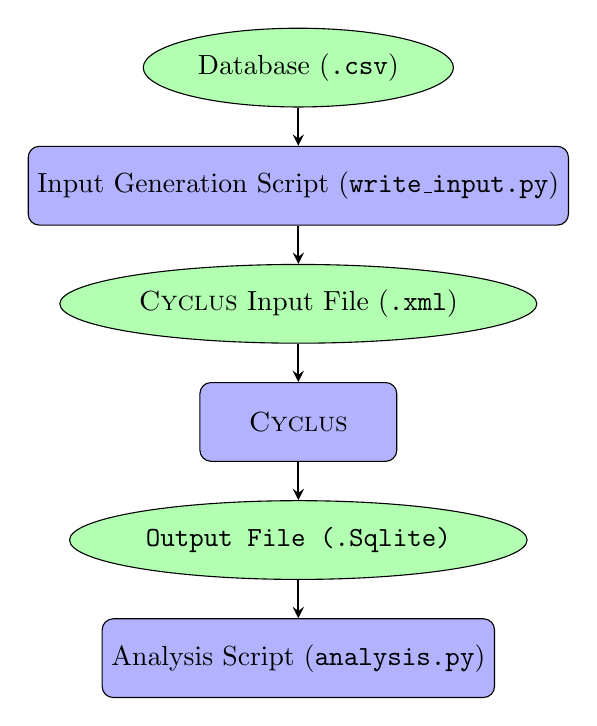
\begin{tikzpicture}[node distance=1.5cm]
\node (database) [object] {Database (\texttt{.csv})};
\node (script) [process, below of=database] {Input Generation Script (\texttt{write\_input.py})};
\node (input) [object, below of=script] {\Cyclus Input File (\texttt{.xml})};
\node (cyclus) [process, below of=input]{\Cyclus};
\node (output) [object, below of=cyclus]{\texttt{Output File (\texttt{.Sqlite})}};
\node (script2) [process, below of=output]{Analysis Script (\texttt{analysis.py})};

\draw [arrow] (database) -- (script); 
\draw [arrow] (script) -- (input); 
\draw [arrow] (input) -- (cyclus);
\draw [arrow] (cyclus) -- (output);
\draw [arrow] (output) -- (script2);
\end{tikzpicture}
\caption{Green circles and blue boxes represent files and software 
processes, respectively, in the computational workflow.}
\label{diag:comp}
\end{figure}


Projections of future reactor deployment in this simulation are based on
assessment of analyses from references, for instance \gls{PRIS}, for reactors planned
for construction \cite{iaea_nuclear_2017}, the World Nuclear Association
\cite{world_nuclear_association_nuclear_2017}, and literature concerning the future of
nuclear power in a global \cite{joskow_future_2012} and European context
\cite{hatch_politics_2015}.  Existing projections extend to 2050.

\Cref{tab:eu_deployment} lists the reactors that are currently  planned or
under construction in the \gls{EU}. In the simulation, all  planned constructions are completed 
without delay or failure and reach a lifetime of 60 years.  

\pagebreak
\begin{table}[h]
    \centering
    \caption {Power reactors under construction and planned. Replicated from \cite{world_nuclear_association_nuclear_2017}.}
    \label{tab:eu_deployment}
    \begin{tabular}{ccccr}
        \hline
        \textbf{Exp. Operational }&\textbf{Country} &\textbf{Reactor} & \textbf{Type} & \textbf{Gross \gls{MWe}}\\
        \hline
        2018 & Slovakia  & Mochovce 3 & PWR & 440\\
        2018 & Slovakia & Mochovce 4 & PWR & 440 \\
        2018 & France & Flamanville 3 & PWR & 1600 \\
        2018 & Finland & Olkilouto 3 & PWR & 1720 \\
        2019 & Romania & Cernavoda 3 & PHWR & 720 \\
        2020 & Romania & Cernavoda 4 & PHWR & 720 \\
        2024 & Finland & Hanhikivi & VVER1200 & 1200 \\
        2024 & Hungary & Paks 5 & VVER1200 & 1200 \\
        2025 & Hungary & Paks 6 & VVER1200 & 1200 \\
        2025 & Bulgaria & Kozloduy 7 & \footnotemark AP1000 & 950 \\
        2026 & UK & Hinkley Point C1 & EPR & 1670 \\
        2027 & UK & Hinkley Point C2 & EPR & 1670 \\
        2029 & Poland & Choczewo & N/A & 3000 \\
        2035 & Poland & N/A & N/A & 3000 \\
        2035 & Czech Rep & Dukovany 5 & N/A & 1200 \\
        2035 & Czech Rep & Temelin 3 & AP1000 & 1200 \\
        2040 & Czech Rep & Temelin 4 & AP1000 & 1200 \\
        \hline
    \end{tabular}
\end{table}

    \footnotetext{The fate of many planned reactors is uncertain. The proposed reactor types
              are also unclear. The ones marked `N/A' for type are assumed to the \glspl{PWR}
              in the simulation.}
\FloatBarrier

For each \gls{EU} nation, we categorize the growth trajectory is categorized from
``Aggressive Growth'' to ``Aggressive Shutdown''. ``Aggressive growth'' is
characterized by a rigorous expansion of nuclear power, while
``Aggressive Shutdown'' is characterized as a transition to rapidly
de-nuclearize the nation's electric grid. We categorize each nation's growth 
trajectory into five degrees depending on G, the growth trajectory metric:

 \[
 G = \left\{\begin{array}{ll}
 \text{Aggressive Growth}, & \text{for } G \geq 2\\
 \text{Modest Growth}, & \text{for } 1.2 \leq G < 2\\
 \text{Maintanence}, & \text{for } 0.8 \leq G < 1.2 \\
 \text{Modest Reduction}, & \text{for } 0.5 \leq G< 0.8\\
 \text{Aggressive Reduction}, & \text{for } G \leq 0.5
 \end{array}\right\} = \frac{C_{2040}}{C_{2017}}\\\\
 \]
 \[
  G = \text{Growth Trajectory  } [-] 
 \]
 \[
 C_{i} = \text{Nuclear Capacity in Year i  } [\gls{MWe}].
 \]

The growth trajectory and specific plan of each nation in the \gls{EU} 
is listed in Table \ref{tab:eu_growth}.  

\begin{table}[h]
    \centering
    \caption{Projected nuclear power strategies of \gls{EU} nations \cite{world_nuclear_association_nuclear_2017}}
        \begin{tabular}{lll}
            \hline 
                    \textbf{Nation} & \textbf{Growth Trajectory} & \textbf{Specific Plan }\\
                    \hline
                    UK & Aggressive Growth & {\small  13 units (17,900 \gls{MWe}) by 2030.}\\
                    Poland & Aggressive Growth &  {\small Additional 6,000 \gls{MWe} by 2035.}\\
                    Hungary & Aggressive Growth &  {\small Additional 2,400 \gls{MWe} by 2025.} \\ 
                    Finland & Modest Growth &  {\small Additional 2,920 \gls{MWe} by 2024.}\\
                    Slovakia & Modest Growth & {\small Additional 942 \gls{MWe} by 2025.}\\
                    Bulgaria & Modest Growth &  {\small Additional 1,000 \gls{MWe} by 2035.} \\
                    Romania & Modest Growth &  {\small Additional 1,440 \gls{MWe} by 2020.} \\
                    Czech Rep. & Modest Growth & {\small  Additional 2,400 \gls{MWe} by 2035.}\\
                    France & Modest Reduction & {\small No expansion or early shutdown.}\\
                    Slovenia & Modest Reduction & {\small No expansion or early shutdown.}\\
                    Netherlands & Modest Reduction & {\small No expansion or early shutdown.}\\
                    Lithuania & Modest Reduction & {\small No expansion or early shutdown.}\\
                    Spain & Modest Reduction &  {\small No expansion or early shutdown.} \\
                    Italy & Modest Reduction & {\small No expansion or early shutdown. }\\
                    Belgium & Aggressive Reduction & All shut down 2025.\\
                    Sweden & Aggressive Reduction & All shut down 2050.\\
                    Germany & Aggressive Reduction & All shut down by 2022.\\
                    \hline
                    
        \end{tabular}

Using this categorization to drive facility deployment, the simulation captures 
regional differences in reactor power capacity and \gls{UNF} production as a 
function of time. Accordingly, \cref{fig:eu_pow} shows the resulting simulated 
installed capacity in \gls{EU} nations.  Sudden capacity reductions seen in the 
2040s result from end-of-license reactor retirements and nuclear phaseout plans 
in nations such as Germany and Belgium.  
    
  \label{tab:eu_growth}
\end{table}
\FloatBarrier

\begin{figure}[htbp!]
    \begin{center}
        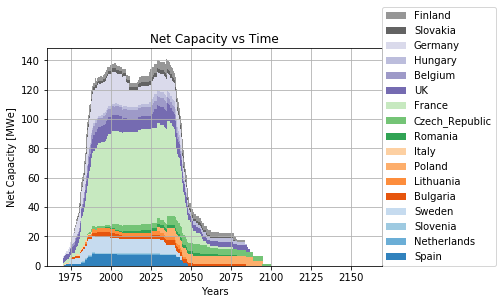
\includegraphics[scale=0.6]{./images/eu_future/power_plot.png}
    \end{center}
    \caption{Installed nuclear capacity in the EU is distinguished by \texttt{Region}s in \Cyclus.}
    \label{fig:eu_pow}
\end{figure}


\subsection{French \gls{SFR} Deployment Schedule}

\Cref{fig:sfr_num}
shows
the French transition to \glspl{SFR} modeled in this simulation.
Historically aggressive growth of nuclear in the 1980s leads to a substantial 
shutdown of nuclear in the 2040s, which, in the simulation, are replaced by new 
\glspl{SFR}. The net capacity is kept constant at 66 GWe.

\begin{figure}[htbp!]
        \begin{center}
                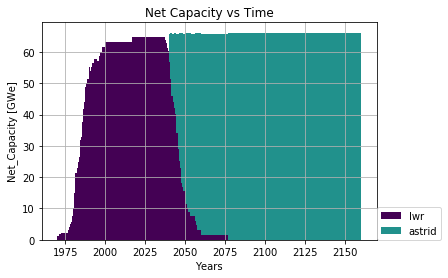
\includegraphics[scale=0.6]{./images/french-transition/power_plot.png}
        \end{center}
        \caption{The potential French transition from \glspl{LWR} to 
                \glspl{SFR} when assisted by \gls{UNF} from other \gls{EU} 
        nations.}
        \label{fig:sfr_num}
\end{figure}

\Cref{fig:dep} shows the deployment required to support the transition in 
\cref{fig:sfr_num}. France must build four reactors per year, on average, to 
make up for the end-of-license decommissioning of power plants built in the 1980s and 1990s.  The second period of aggressive building occurs when the first generation of \glspl{SFR} decommission after 80 years. Starting in 2040, France deploys 600-\gls{MWe} \glspl{SFR} to make up for 
decommissioned French \gls{LWR} capacity. This results in an installed 
\gls{SFR} 
capacity of 66,000 \gls{MWe} by 2078 when the final \gls{LWR} is 
decommissioned. 



\begin{figure}[htbp!]
    \begin{center}
        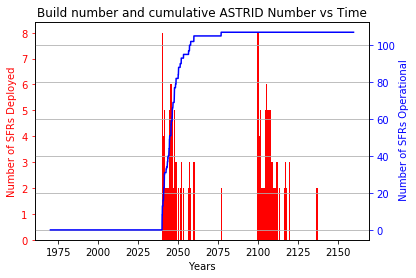
\includegraphics[scale=0.6]{./images/french-transition/sfr_deploy.png}
    \end{center}
    \caption{The deployment of \glspl{SFR} in France is characterized by a period of
    aggressive building.}
    \label{fig:dep}
\end{figure}


Finally, \Cref{fig:tot_dep} shows the total deployment scheme we simulated.  
The French transition to \glspl{SFR} couples with the historical and projected 
operation of \gls{EU} reactors.  The steep transition from 2040 to 2060 
reflects the scheduled decommissioning of reactors built in the 1975-2000 era 
of aggressive nuclear growth in France.

\begin{figure}[htbp!]
    \begin{center}
        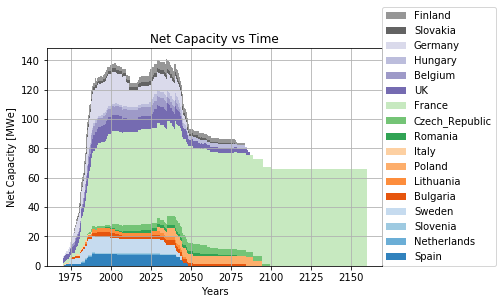
\includegraphics[scale=0.6]{./images/eu_future/onesim.png}
    \end{center}
    \caption{The total deployment scheme we simulated relies on \gls{UNF} 
    collaboration among nations.} 
    \label{fig:tot_dep}
\end{figure}

These figures reflect that, for the given assumptions, bursts of construction
are necessary to maintain capacity.  In reality, a construction rate of five 
reactors every year is ambitious, but might have the advantage of
larger scale production of components and more modular assembly and construction if major components can mostly be built off site.

This analysis establishes a multi-national material flow and demonstrates that, if such an aggressive deployment scheme took place, the \glspl{SFR} would have enough fuel.

\subsection{Scenario Specification}

The scenario specifications defining the simulations presented in this work 
are listed in table \ref{tab:gen}.
The reprocessing and \gls{MOX} fabrication capacity in France
prior to 2020 is modeled after the 
French La Hague and MELOX sites \cite{schneider_spent_2008, hugelmann_melox_1999}.


\begin{table}[h]
    \centering
    \caption{Simulation Specifications}
    \begin{tabularx}{\linewidth}{bss}
        \hline
        \textbf{Specification} &\textbf{ Value} & \textbf{Units}\\
        \hline
        Simulation Starts & 1970 & year\\
        Simulation Ends & 2160 & year\\ 
        Production of \gls{ASTRID} fuel begins & 2020 & year\\
        \glspl{SFR} become available & 2040 & year\\
        Reprocessed uranium usage &  Not used anywhere & -\\
        Minimum \gls{UNF} cooling time  & 36  & months\\
        Separation efficiency of U and Pu & 99.8 & \% \\
        Reprocessing streams & Pu and U & - \\
        Reprocessing capacity before 2020 & 91.6 \cite{schneider_spent_2008} & $\frac{\text{metric tons of \gls{UNF}}}{month}$  \\
        Reprocessing capacity after 2020 & 183.2 & $\frac{\text{metric tons of \gls{UNF}}}{month}$\\
        \gls{LWR} \gls{MOX} fabrication throughput & 16.25 \cite{hugelmann_melox_1999} & $\frac{\text{metric tons of \gls{MOX}}}{month}$\\
        \gls{ASTRID} \gls{MOX} fabrication throughput & No limit ($\infty$) & $\frac{\text{metric tons of \gls{MOX}}}{month}$ \\
        \gls{LWR} \gls{MOX} recycling  &  Not reprocessed & - \\
        \gls{ASTRID} \gls{MOX} recycling & $\infty$-pass & - \\
        \hline
    \end{tabularx}
    \label{tab:gen}
\end{table}


\pagebreak

\section{Reactor Specifications}
Three major reactors are used in the simulation, \gls{PWR}, \gls{BWR}, and ASTRID-type \gls{SFR} reactors.


For \glspl{LWR}, we used a linear core size model to capture
varying reactor capacity. For example, a 
1,200 \gls{MWe} PWR has $193*\frac{1,200}{1,000} = 232$ \gls{UOX} assemblies, each
weighing 523.4 kg.
After each 18 month cycle, one-third of the 
core (77 assemblies) discharges. Refueling
is assumed to take two months to complete, during which the reactor
is shut down. The specifications are defined in table \ref{tab:reactor-specs} 
which details the reactor specifications in this simulation. \gls{LWR} 
specifications are modified linearly for varying power capacity.  

\begin{table}[h]
    \centering
    \caption{Baseline \gls{LWR} and \gls{ASTRID} simulation specifications.}
    \begin{tabular}{lrrr}
        \hline
        \textbf{Specification} & \textbf{\gls{PWR} \cite{sutharshan_ap1000tm_2011}} & \textbf{\gls{BWR} \cite{hinds_next-generation_2006}} & \textbf{\gls{SFR}} \cite{varaine_pre-conceptual_2012}\\
        \hline
                Lifetime [y] \tablefootnote{The simulated reactor lifetime reaches the licensed lifetime unless 
        the reactor is shut down prematurely.} & 60 & 60 & 80 \\
                Cycle Time [mos.]& 18 & 18 & 12\\ 
                Refueling Outage [mos.]& 2 & 2  & 2\\
                Rated Power [\gls{MWe}] & 1000 & 1000 & 600\\
                Assembly mass [kg] & 523.4 & 180 & -- \\
                Batch mass [kg] & -- & -- & 5,568\\
                Discharge Burnup [GWd/tHM] & 51 & 51 & 105 \\
                Assemblies per core \tablefootnote{Number of assemblies and corresponding \gls{LWR} core 
        masses are reported for a 1000-\gls{MWe} core. Reactors with different core  
        powers are modeled with a linear mass assumption.} & 193  & 764 & -- \\

                Batches per core & 3 & 3 & 4\\
        Initial Fissile Loading [t] & 3.1  $^{235}$U & 4.2  $^{235}$U & 4.9 Pu \\
                Fuel & \gls{UOX} or \gls{MOX} & \gls{UOX} & \gls{MOX} \\
        \hline
    \end{tabular}
        
    \label{tab:reactor-specs}

    \end{table}


\subsection{Material Definitions}
Depletion calculations of the nuclear fuel are recipe-based, such that a fresh 
and used fuel recipe is defined for each reactor type.
For the compositions of the used fuel, a reference depletion calculation
from ORIGEN is used (see \cref{tab:comp}). ORIGEN calculates buildup,
 decay, and processing of radioactive materials
\cite{parks_overview_1992}. This recipe recipe has also been used for repository performance modeling \cite{wilson_adoption_2009}.

\begin{table}[h]
    \centering
    \caption{Fresh fuel compositions in the simulation \cite{wilson_adoption_2009, varaine_pre-conceptual_2012}.}
%   \scalebox{0.86}{
        \begin{tabular}{lrrr}
            \hline
             & \multicolumn{3}{c}{ Composition [\%]} \\
            Recipe & U-235  & U-238  & Pu \\ 
            \hline
            Fresh \gls{UOX} Fuel & 3.1 & 96.9 & -   \\ 
            Fresh \gls{LWR} \gls{MOX} Fuel & 0.2 & 90.7 & 9.1 \\ 
            Fresh \gls{ASTRID} Fuel & 0.2 & 77.7 & 22 \\
            \hline
        \end{tabular}
        
        \label{tab:sim_result}
\end {table}



\subsection{Results - Transition Scenario}
This section displays the simulation results if France utilized
\gls{UNF} from other \gls{EU} nations to fuel the transition into a fully
\glspl{ASTRID} fleet.

\subsubsection{Nuclear Fuel Material Inventory}
\Cref{tab:sim_result1} 
lists \gls{EU} material inventory in 2050.
The materials continue to accumulate after 2050, but the
\gls{UNF} France receives before 2050 is most impactful for the
feasibility of the transition. Note that \cref{tab:sim_result1} 
distinguishes the
\gls{UOX} in the simulation either stored or reprocessed to create \gls{MOX}.


\begin{table}[h]
    \centering
        \caption{\gls{EU} nuclear material inventory in 2050.}
\begin{tabularx}{\textwidth}{XrX}
            \hline
                        \textbf{Category} & \textbf{Value} & Specifics \\
                                          & \textbf{[MTHM]} & \\ \hline
                        UOX Loaded  & 161,894 & UOX used in EU (minus France) reactors 1970-2050\\ 
            MOX Loaded  & 6,945  & MOX used in French reactors 1970-2050\\
                        Available used UOX (EU)  & 95,193  & Used EU (minus France) 
                                UOX in storage for future ASTRID MOX 
                                production\\
                        Available used UOX (France) & 
                                10,029  & Used French UOX stored for 
                                future ASTRID MOX production. \\
                                Reprocessed UOX (France) & 53,590 & Used French UOX already reprocessed for the production of LWR MOX \\
            Tails  & 980,294  & (Tails generated) $-$ (Tails used for production of LWR MOX) \\ 
            Natural U Used  & 1,142,189  & \\ \hline
        \end{tabularx}
        
        \label{tab:sim_result1}
\end {table}
\FloatBarrier


Figures \ref{fig:eu_tail} and \ref{fig:eu_snf} show the 
accumulation of tails and used fuel over time in the \gls{EU}.
Tails accumulate as a by-product of uranium enrichment. For every
ton of \gls{UOX} fuel, about nine times of tails is produced. 
Spent fuel is discharged from reactors every refueling period.
The entire core is discharged when the reactor decommissions.
A total of about $1,000,000$ MTHM of tails and $100,000$ MTHM of
\gls{UNF} have accumulated by 2050.
Figure \ref{fig:eu_fuel} shows the amount of fuel used in the \gls{EU}. The 
tails mass accumulation rate is fairly steady, with peaks occurring when new 
reactors are deployed.
In \cref{fig:eu_snf}, the peaks are caused by reactor decommissioning which 
triggers all the batches in the final reactor core to be sent to the repository.

\begin{figure}[htbp!]
    \begin{center}
        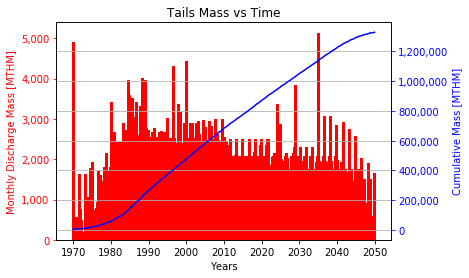
\includegraphics[scale=0.7]{./images/eu_future/tails.png}
    \end{center}
        \caption{Simulated accumulation of tails in the \gls{EU} is shown as a function of time.}
    \label{fig:eu_tail}
\end{figure}

\begin{figure}[htbp!]
    \begin{center}
        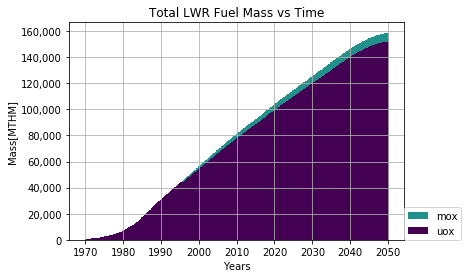
\includegraphics[scale=0.7]{./images/eu_future/total_fuel.png}
    \end{center}
\caption{Simulated total \gls{EU} fuel useage is shown as a function of time.}
    \label{fig:eu_fuel}
\end{figure}


\begin{figure}[htbp!]
    \begin{center}
            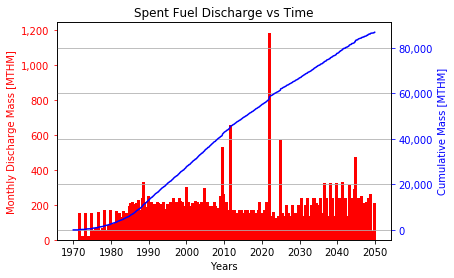
\includegraphics[scale=0.7]{./images/eu_future/snf_discharge.png}
    \end{center}
        \caption{Simulated \gls{EU} \gls{UNF} accumulation and discharge is 
shown as a function of time.}
    \label{fig:eu_snf}
\end{figure}


\subsubsection{French \gls{SFR} Deployment}
\FloatBarrier

Reprocessing the \gls{UNF} collected from all EU nations can provide the 
initial cores for approximately 180 \glspl{SFR}. Table \ref{tab:pu} lists the 
isotope, mass fraction, and quantity of plutonium that can be obtained from the 
2050 \gls{UNF} inventory.  With the \gls{SFR} breeding ratio above one, France 
can transition into a fully \gls{SFR} fleet without extra construction of 
\glspl{LWR}. 

\begin{table}[h]
    \centering
    \caption{Plutonium in the \gls{UNF} inventory.}
    \begin{tabular}{lrr}
        \hline
        \textbf{Isotope} & \textbf{Mass Fraction in Used Fuel [\%]} & \textbf{Quantity [t]} \\ \hline
        Pu238 & 0.0111 & 10.52 \\ 
        Pu239 & 0.518 & 545.05 \\ 
        Pu240 & 0.232 & 244.11 \\ 
        Pu241 & 0.126 & 132.58 \\ 
        Pu242 & 0.0487 & 51.24 \\ \hline
        \textbf{Total} & \textbf{0.9358} & \textbf{983.52} \\ \hline
    \end{tabular}
    
    \label{tab:pu}
\end{table}

From Varaine et al. \cite{varaine_pre-conceptual_2012}, a French
ASTRID-type 600\gls{MWe} \gls{SFR} consumes $1.225$ metric tons of
plutonium a year, with an initial plutonium loading of $4.9$ metric tons. 
Thus, the number of \glspl{SFR} that can be loaded with the reprocessed
plutonium from \gls{UNF} can be estimated to be 200, assuming adequate 
reprocessing and fabrication capacity as well as abundant depleted uranium 
supply.
 
Used \gls{MOX} from an ASTRID reactor is 23.95\% plutonium
in this simulation (see \cref{tab:comp}), whereas fresh \gls{MOX} is 22\% plutonium.
The plutonium breeding ratio in this simulation is thus assumed to be
$\approx 1.08$.

\Cref{fig:fuel} shows \gls{MOX} loaded in the \glspl{SFR} per month.  The plot 
has peaks during a period of aggressive deployment of \glspl{SFR} followed by 
an equilibrium at 100 \gls{MTHM}. The peaks reoccur with the deployment of the 
second generation of \glspl{SFR}.  The spikes are due to initial fuel demand 
correspoding to these new deployments.  The initial cores loaded into new 
\glspl{SFR} rely on the \gls{MOX} created from legacy \gls{UNF}. Once the 
deployed \glspl{SFR} create enough extra plutonium, the legacy \gls{UNF} is no 
longer used. Notably, this switch from a less preferred fuel origin to a more 
preferred fuel origin is handled automatically within \Cyclus via user-defined preferences 
within its dynamic resource exchange algorithm \cite{gidden_methodology_2016}.


\begin{figure}[htbp!]
    \begin{center}
        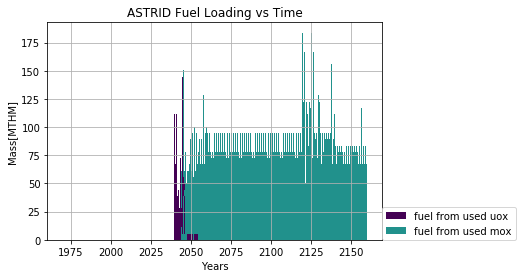
\includegraphics[width=0.7\textwidth]{./images/french-transition/where_fuel.png}
    \end{center}
    \caption{Fuel loaded into \glspl{SFR} was simulated in discrete 
        batches.}
    \label{fig:fuel}
\end{figure}

\Cref{fig:pu_no_cum} shows the separated plutonium discharge per month from the reprocessing plant. The plutonium outflux does not precisely follow the fuel demand because \Cyclus agents have material buffers that store commodity fuel for later usage. The reprocessed plutonium from legacy \gls{UNF} is stored for the initial loading of \glspl{SFR}.  Plutonium separated from legacy \gls{UNF} meets plutonium demans sufficiently to reduce the reprocessing demand for the first aggressive deployment of \glspl{SFR}.  The plutonium from reprocessing legacy fuel is a flat rectangle because the reprocessing throughput was set to 183.2 $\frac{\gls{MTHM}}{month}$ to avoid reprocessing all the legacy in one timestep. 
 

\begin{figure}[htbp!]
    \begin{center}
        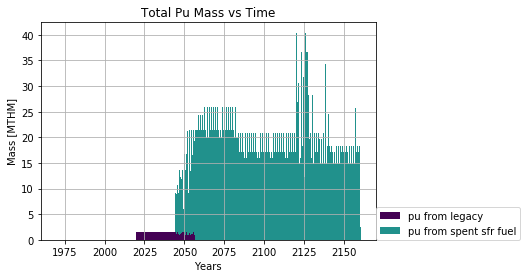
\includegraphics[scale=0.7]{./images/french-transition/pu.png}
    \end{center}
    \caption{The separated plutonium discharge from the reprocessing plant 
        in $\frac{\mbox{MTHM}}{\mbox{month}}$.}
    \label{fig:pu_no_cum}
\end{figure}

 \Cref{tab:sfr_sim_result} lists metrics obtained from the second simulation.

\begin{table}[h]
    \centering
    \caption {In the French transition to \glspl{SFR},
                  the total legacy \gls{UNF} reprocessed is the 
                                  amount of \gls{UNF} France needs 
                  for a transition into a fully \gls{SFR} fleet. 
                                  %The tails used is around ninth of the original tails inventory from the previous simulation.
                                  %KDH note: What does this mean?
                                  %thought there was only one simulation. . . 
                          }
    \scalebox{0.86}{
        \begin{tabular}{llr}
            \hline
            \textbf{Category} & \textbf{Unit} & \textbf{Value}  \\ \hline
            Total \gls{ASTRID} MOX used & MTHM & 63,447  \\ 
            \textbf{Average UOX Reprocessing} & MTHM/month & \textbf{123.27} \\
            \textbf{Average Total Reprocessing} & MTHM/month & \textbf{63.23} \\
            \textbf{Average Fuel Fabrication} & MTHM/month & \textbf{74.31} \\
            Total \glspl{SFR} Deployed & & 220 \\ 
            Total Plutonium Reprocessed & MTHM & 14,831 \\ 
            Total \gls{ASTRID} fuel from UOX Waste & MTHM & 2,895  \\ 
            Total \gls{ASTRID} fuel from MOX Waste & MTHM  & 60,552 \\ 
            Total Tails used & MTHM & 49,488 \\ 
            \textbf{Total legacy UNF reprocessed} & MTHM & \textbf{53,595} \\ 
            Total Reprocessed Uranium Stockpile & MTHM & 159,383 \\ 
            Total Raffinate & MTHM & 24,789 \\ \hline
        \end{tabular}}
        
        \label{tab:sfr_sim_result}
\end {table}


These results demonstrate that despite the large amount of initial plutonium that has to be reprocessed
prior to \gls{ASTRID} deployment, the 20 years (2020-2040) of 
\gls{ASTRID} fuel preparation
allows a reasonable level of average
\gls{UOX} reprocessing capacity demand. \gls{UOX} reprocessing continues 
until 2057, when the \gls{ASTRID} spent fuel can supply the plutonium
for its own fuel.

\subsubsection{Conclusion}

France can transition into
a fully \gls{SFR} fleet with installed capacity of 66,000 \gls{MWe} without
building additional \glspl{LWR}
if France receives \gls{UNF} from other \gls{EU} nations.
Supporting the \gls{SFR} fleet requires an average 
reprocessing capacity of 73.27 \gls{MTHM} per month,
and an average fabrication capacity of 45.29 \gls{MTHM} per month.

Since most \gls{EU} nations do not have an operating \gls{UNF}
repository or a management plan, they have a strong incentive
to send their \gls{UNF} to France. In particular, the nations
planning aggressive nuclear reduction will be able phase out nuclear
without constructing a permanent repository. France has an
incentive to take this fuel, since recycling used fuel from
other nations will allow France to meet their MOX demand
without new construction of \glspl{LWR}.

\Cref{tab:which_send} lists \gls{EU} nations and their \gls{UNF} inventory
in 2050. We analyzed a strategy in which 
the nations reducing their nuclear fleet send their \gls{UNF} to France.
The sum of \gls{UNF} from Italy, Slovenia, Belgium, Spain and Germany
provides enough \gls{UNF} for the simulated transition ($\approx 54,000$ MTHM). 
These nations are shown in bold in \cref{tab:which_send}.
Sweden is not considered because of its concrete waste management plan.


\begin{table}[h]
    \centering
    \caption {\gls{EU} nations and their respective \gls{UNF} inventory.} 
                \begin{tabularx}{\textwidth}{llr}
                    \hline 
                    \textbf{Nation} & \textbf{Growth Trajectory} & \small{\textbf{UNF in 2050 [MTHM] }}\\
                    \hline
                    Poland & Aggressive Growth & 1,807\\
                    Hungary & Aggressive Growth & 3,119 \\ 
                    UK & Aggressive Growth & 13,268\\
                    Slovakia & Modest Growth & 2,746\\
                    Bulgaria & Modest Growth & 3,237 \\
                    Czech Rep. & Modest Growth & 4,413\\
                    Finland & Modest Growth &  5,713\\
                    Netherlands & Modest Reduction & 539\\
                    \textbf{Italy} & \textbf{Modest Reduction} & \textbf{583}\\
                    \textbf{Slovenia} & \textbf{Modest Reduction} & \textbf{765}\\
                    \textbf{Lithuania} & \textbf{Modest Reduction} & \textbf{2,644} \\
                    \textbf{Belgium} & \textbf{Aggressive Reduction} & \textbf{6,644}\\
                    \textbf{Spain} & \textbf{Modest Reduction} &  \textbf{9,771} \\
                    \textbf{France} & \textbf{Modest Reduction} & \textbf{9,979} \\
                    Sweden & Aggressive Reduction & 16,035\\
                    \textbf{Germany} & \textbf{Aggressive Reduction} & \textbf{23,868}\\
                    \hline
                \end{tabularx}
    
    \label{tab:which_send}

\end{table}

On the other hand, in these simulations, some complex political and economic factors were not incorporated and various assumptions were present in this scenario. For
example, Germany's current policy is to not reprocess its \gls{LWR} fuel
\cite{topfer_germanys_2011}, and this policy would create a shortage
in the supply of \gls{LWR} \gls{UNF} for \gls{ASTRID} \gls{MOX} production.
Continuation of that German policy would not, however, be incompatible
with a change in \gls{EU} policy that frees \gls{EU} countries from
creating their high level waste repositories, since France could still
agree to take in Germany's \gls{UNF} for direct disposal. The analysis
method described herein could readily be adapted to account for such possibilities. 
The collaborative option explored here may hold value for the \gls{EU} nuclear community,
and may enable France to advance more rapidly into a closed fuel cycle. 
\FloatBarrier


\subsection{Results - Maintain Status Quo}





\section{United States}
The United States have been the forerunner of nuclear energy, with a current
installed capacity of about 100 GWe. With its size and long history of nuclear
energy, the United States have accumulated about $70,000$ \gls{MTHM} of \gls{UNF}.
The United States' historical nuclear operation and inventory is tracked using
\Cyclus and is compared with benchmarked results from \gls{ORION} and the
\gls{UNF-STANDARDS} database. The \gls{UNF-STANDARDS} database is a comprehensive,
controlled source of \gls{UNF} information, including dry cask attributes, assembly
data, and economic attributes \cite{peterson_unf_2017}. With the successful benchmark,
the simulation is be extrapolated to the future. Two separate simulations, one with
transition into a `closed' fuel cycle, and the other once-through, is run.

The problem with modeling the U.S. transition scenario is that the U.S. does not have
a defined advanced reactor, whereas France has a solid plan to transition into \glspl{ASTRID}.

This chapter includes the results and comparison of two simulations:
\begin{enumerate}
    \item The United States transitions into a `closed' fuel cycle with breeder reactors and reprocessing.
    \item The United States maintains once-through cycle.
\end{enumerate}



\section{\gls{UDB} Reactor Module}

The logic flow of the UDB reactor module is illustrated in figure \ref{fig:logic}.

\tikzstyle{decision} = [diamond, draw, fill=blue!20, 
    text width=5em, text badly centered,  inner sep=0pt]
\tikzstyle{block} = [rectangle, draw, fill=blue!20, 
    text width=8em, text centered, rounded corners, minimum height=3em]
\tikzstyle{buff} = [rectangle, draw, fill=green!20, 
    text width=8em, text centered, rounded corners, minimum height=3em]
\tikzstyle{kernal} = [rectangle, draw, fill=red!20, 
    text width=8em, text centered, rounded corners, minimum height=3em]
\tikzstyle{line} = [draw, -latex']
\tikzstyle{dummy} = [rectangle]
\tikzstyle{cloud} = [draw, text centered, ellipse,fill=red!20, text width=15em,
    minimum height=2em]

\usetikzlibrary{calc}

\begin{figure}[!ht]
\begin{tikzpicture}[node distance = 2.5cm and 2cm, auto]
    % Place nodes
    \node [kernal] (enternotify) {Set buy policy};
    \node [block, below of=enternotify] (tick1) {Empty tick?};
    \node [kernal, below of=tick1] (dre) {DRE - receive fuel and fill};
    \node [decision, below of=dre] (core?) {Is core Loaded?};
    \node [block, right = of dre] (tock) {Shutdown State - Do nothing};
    \node [decision, below of=core?] (crit1) {Critical?};
    \node [block, left = of crit1] (fiss) {Ask for more fissile?};
    \node [block, below of=crit1] (dep) {Deplete using ROM};
    \node [buff, below of=dep] (torep) {Core to Rep};
    \node [block, right = of torep] (rep) {Separate};
    \node [buff, below of=torep] (refill) {Refill Core from fill tank};
    \node [buff, right = of dep] (waste) {Add separated waste to waste for market};
    \node [buff, right = of refill] (backto) {Send fuel isotope back into core};
    \node [buff, right = of rep] (patank) {Pa tank for decay};
    \node [block, right = of backto] (decay) {Decay until Useful};
    \node [decision, below of=refill] (crit2) {Critical?};
    \node [buff, below of=decay] (backto2) {Send fuel isotope back into core};


    % Draw edges
    \path [line] (enternotify) -- (tick1);
    \path [line] (tick1) -- (dre);
    \path [line] (core?) -| node [near start] {no} (tock);
    \path [line] (tock) |- (tick1);
    \path [line] (dre) -- (core?);
    \path [line] (core?) -- node {yes} (crit1);
    \path [line] (crit1) -- node {yes} (dep);
    \path [line] (crit1) -- node {no} (fiss);
    \path [line] (dep) -- (torep);
    \path [line] (torep) -- (refill);
    \path [line] (refill) -- (crit2);
    \path [line] (torep) -- (rep);
    \path [line] (rep) -- (waste);
    \path [line] (rep) -- (patank);
    \path [line] (rep) -- (backto);
    \path [line] (backto) -- (crit2);
    \path [line] (patank) -- (decay);
    \path [line] (decay) -- (backto2);
    \path [line] (backto2) -- (crit2);
    \path [line] (crit2.south) |- node {no} ($(crit2.south) - (0,5mm)$) -|  (fiss);
    \path [line] (crit2.west) -| node {yes} ($(crit2.west) - (10mm, 0)$) |-  (dep);
    

    

    %\path [line] (decide) -| node [near start] {yes} (update);
    %\path [line] (update) |- (identify);
    %\path [line] (decide) -- node {no}(stop);
    \end{tikzpicture}
\caption{\color{red}{Kernal Interactions}, \color{blue}{In-agent functions}, 
         \color{green}{Buffer Transactions}.}
\label{fig:logic}
\end{figure}

%\chapter{Conclusions}


%\appendix*
%\include{Appendix.tex}

\section{Fuel Cycles to Compare}

\bibliographystyle{unsrtnat}
\bibliography{bibliography}


\end{document}
\endinput
%%
%% End of file `thesis-ex.tex'.
